\documentclass[11pt]{article}

\usepackage[margin=1in]{geometry}
\usepackage{amsmath, amssymb}
\usepackage{bm}
\usepackage{booktabs}
\usepackage{graphicx}
\usepackage{enumitem}
\usepackage{float}
\usepackage{xcolor}
\usepackage{parskip}
\usepackage[hidelinks]{hyperref}

\setlist{itemsep=2pt, topsep=4pt}
\newcommand{\code}[1]{\begingroup\renewcommand{\_}{\textunderscore\allowbreak}\texttt{#1}\endgroup}  % file names may break after underscores
\setlength{\emergencystretch}{3em}

\title{Finding Existing Merchants to Start Using Subscriptions}
\author{Yiyi Huo}
\date{October 2026}

\begin{document}

\maketitle

%--------------------------------------------------------------------
\section*{Background}

This project uses simulated data previously provided by a company: a sample of merchants with daily payment volume for three products (Subscriptions, Checkout, Payment Links) and a merchant profile. The goal was to build a quantitative approach that picks existing merchants for a campaign to adopt Subscriptions.

In summary:
\begin{itemize}
  \item \textbf{Prediction target.} Whether a merchant not yet using Subscriptions starts using it in the next 90 days.
  \item \textbf{Approach.} A logistic regression and a random forest on monthly snapshots, with covariates from past data only. The final ranking averages the two models' ranks.
  \item \textbf{Validation.} Tested on a later held-out snapshot: AUC 0.73, and 9\% of the top 100 merchants adopt vs a 1\% base rate.
\end{itemize}

%--------------------------------------------------------------------
\section{Goal}\label{sec:goal}

Our goal is to identify, among merchants who have not yet adopted Subscriptions, those most likely to adopt it soon, so that sales or marketing campaigns can focus on them. We frame this as a probability estimation problem. For merchant $i$ with covariates $X_i$ (its profile and payment behavior), let $Y_i = 1$ indicate whether it adopts Subscriptions. We model
\begin{align*}
p_i = P(Y_i = 1 \mid X_i),
\end{align*}
and the campaign list consists of the merchants with the highest estimated $\hat p_i$. The exact definitions of $X_i$ and $Y_i$, and how they relate to time, are given in Section~\ref{sec:logit}.

We mainly consider two approaches:
\begin{itemize}
  \item \textbf{Logistic regression} on monthly rolling snapshots (main model).
  \item \textbf{Random forest} on the same snapshots, tuned by time-series cross-validation.
\end{itemize}
The final ranking is an equal-weight combination of the two.

Along the way we also considered a logistic regression without time (merchants that ever vs never used Subscriptions), L1 and L2 regularized logistic regressions, other tree models and a GAM, and hazard models (discrete-time, Cox and time-varying Cox); Sections~\ref{sec:logit} and~\ref{sec:rf} explain why we chose the two models above, Section~\ref{sec:combine} how we combine them, and Section~\ref{sec:hazard} discusses the hazard models.

%--------------------------------------------------------------------
\section{Data}\label{sec:data}

We received two datasets: \textbf{merchants} (merchant profiles) and \textbf{payments} (daily payment volume per merchant and product). For cleaning, we did the following:
\begin{enumerate}
  \item \textbf{Formats.} We checked and standardized the format of every column, including merchant ids, dates, and volumes (cents to dollars).
  \item \textbf{Invalid rows.} We removed invalid records, such as duplicated ids and id \code{0}.
  \item \textbf{Missing values.} We recoded placeholder values as missing.
\end{enumerate}
Details of each check are in \code{data\_cleaning.ipynb}.

After merging the two datasets into one row per merchant, we examined the candidate covariates and their raw distributions (Table~\ref{tab:summary}).

\begin{table}[H]
\centering
\caption{Summary of the candidate covariates, one row per merchant.}
\label{tab:summary}
\resizebox{\textwidth}{!}{%
\begin{tabular}{llrrllllll}
\toprule
Variable & Type & Missing & Levels & Min & 25\% & 50\% & 75\% & 99\% & Max \\
\midrule
industry & category & 7 & 29 & & & & & & \\
country & category & 0 & 44 & & & & & & \\
business\_size & category & 0 & 3 & & & & & & \\
first\_charge\_date & date & 26 & & 2030-11-07 & 2039-06-25 & 2040-12-06 & 2041-09-22 & 2042-06-13 & 2042-06-22 \\
first\_seen & date & 0 & & 2041-05-01 & 2041-05-04 & 2041-06-20 & 2041-11-24 & 2042-06-15 & 2042-06-22 \\
last\_seen & date & 0 & & 2041-05-01 & 2042-01-26 & 2042-05-31 & 2042-06-20 & 2042-06-22 & 2042-06-22 \\
active\_days & integer & 0 & & 1 & 3 & 14 & 73 & 418 & 418 \\
non\_sub\_volume & numeric & 0 & & 0 & 136 & 1,794 & 14,944 & 1,604,969 & 989,263,610 \\
checkout\_volume & numeric & 0 & & 0 & 0 & 0 & 0 & 96,423 & 16,267,923 \\
payment\_link\_volume & numeric & 0 & & 0 & 0 & 0 & 0 & 20,737 & 1,212,347 \\
\bottomrule
\end{tabular}%
}
\end{table}

We use \textbf{3 discrete covariates} (industry, country, business size) and \textbf{6 continuous covariates} (volume, Checkout volume, Payment Links volume, active rate, recency, tenure). Based on these distributions, we made the following changes:
\begin{itemize}
  \item \textbf{Merge small classes} (less than 5\% of merchants):
  \begin{itemize}
    \item Industry: small industries and missing values are merged into Others.
    \item Country: small countries are grouped into three regions (Western \& Northern Europe, Southern \& Eastern Europe, Rest of world).
    \item Business size: medium and large are merged into one class.
  \end{itemize}
  \item \textbf{Log-transform volumes:}
  \begin{itemize}
    \item Volume, Checkout volume and Payment Links volume are transformed to $\log(1 + \text{volume})$.
  \end{itemize}
  \item \textbf{Define activity covariates} from \code{active\_days}, \code{first\_seen} and \code{last\_seen}:
  \begin{itemize}
    \item Active rate is defined as the number of active days divided by the number of days observed.
    \item Recency is defined as the number of days since the last payment.
  \end{itemize}
  \item \textbf{Define tenure} from \code{first\_charge\_date}:
  \begin{itemize}
    \item Tenure is defined as the number of days from the first charge date to the snapshot date, and enters as $\log(\text{tenure})$.
  \end{itemize}
\end{itemize}

The reasons for these changes are:
\begin{itemize}
  \item \textbf{Small industry and business size classes.} We merged small classes because adoption is rare, so a small class contains only a few adopters and its coefficient is estimated with a lot of noise. Adding more dummy variables would increase the variance of the model without making its predictions more accurate.
  \item \textbf{Countries by geography.} We grouped small countries into geographic regions instead of a single Others class because this keeps the meaning of the covariate, adjusting for regional differences, while still avoiding the small-class issue above.
  \item \textbf{Log volumes.} We log-transformed the volumes because the summary table shows they are extremely right-skewed, with many zeros and a few very large merchants. On the log scale the distribution is much less skewed, which suits the linear predictor of the logistic regression used later.
  \item \textbf{Activity covariates.} \code{active\_days}, \code{first\_seen} and \code{last\_seen} can be combined in several ways, for example active days with days observed, or the raw first and last payment dates. We chose the active rate and recency for two reasons. First, they have a clear meaning at any snapshot, whereas raw first and last payment dates are calendar dates whose meaning changes with the snapshot date. Second, they have low correlation with each other, whereas active days and days observed are strongly correlated because active days grow with the time a merchant has been observed.
  \item \textbf{Tenure.} We log-transformed tenure because it is right-skewed, and adoption drops fastest in a merchant's first months.
\end{itemize}
Details of the distributions and of these changes, including the class tables and histograms of each variable, are in \code{covariates.ipynb}.

%--------------------------------------------------------------------
\section{Logistic regression}\label{sec:logit}

A natural starting point for this problem is a simple linear model, such as a \textbf{plain logistic regression}, where $Y_i = 1$ if merchant $i$ ever adopted Subscriptions and covariates are aggregated over the entire observation period. However, this approach has several limitations.
\begin{itemize}
  \item \textbf{Data leakage.} Covariates computed over the entire period may include post-adoption information.
  \item \textbf{Time-varying covariates.} Important predictors such as transaction volume, activity and recency change over time, so aggregating them into a single value loses temporal information.
  \item \textbf{Need for adjustment.} Dropping these time-dependent covariates would discard important information for predicting adoption.
\end{itemize}

Therefore, we use a \textbf{time-varying logistic regression} to account for changes in merchant characteristics over time while avoiding data leakage:
\begin{align*}
\log \frac{P(Y_{it} = 1 \mid X_{it})}{1 - P(Y_{it} = 1 \mid X_{it})} = \beta_0 + \beta^\top X_{it},
\end{align*}
where
\begin{itemize}
  \item $t$ is a snapshot date, the first day of each month;
  \item $Y_{it} = \mathbf{1}\{t \le A_i < t + H\}$ indicates adoption within $H$ days after $t$, with $A_i$ the first day merchant $i$ uses Subscriptions;
  \item $X_{it}$ are the covariates of Section~\ref{sec:data}, computed only from the window $[t - H, t)$, so no future information enters;
  \item the sample at each $t$ is the merchants observed for at least $L$ days that do not use Subscriptions yet and were active in $[t - H, t)$.
\end{itemize}

\paragraph{Parameters.} We chose $H$ and $L$ from a \textbf{grid of values}, comparing the number of training snapshots, the adoption rate and the number of adopters, and set:
\begin{itemize}
  \item $H = 90$ days (horizon and covariate window);
  \item $L = 30$ days (minimum history).
\end{itemize}

\paragraph{Training and testing (rolling snapshots).}
\begin{itemize}
  \item \textbf{Training:} monthly snapshots whose outcome windows end before the test snapshot, stacked.
  \item \textbf{Test:} one snapshot $H$ days before the end of the data, not used for fitting.
\end{itemize}
Table~\ref{tab:example} shows an example of the stacked training data.

\begin{table}[H]
\centering
\caption{Example of the stacked training data.}
\label{tab:example}
\begin{tabular}{lllrrrr}
\toprule
Merchant & Snapshot $t$ & Industry & log volume & Active rate & Recency & $Y_{it}$ \\
\midrule
A & 2041-08-01 & Software & 7.30 & 0.03 & 2 & 0 \\
A & 2041-09-01 & Software & 7.01 & 0.02 & 24 & 1 \\
A & 2041-10-01 & Software & 8.34 & 0.04 & 0 & 1 \\
A & 2041-11-01 & Software & 8.77 & 0.06 & 16 & 1 \\
B & 2041-08-01 & Software & 10.11 & 0.13 & 5 & 0 \\
B & 2041-09-01 & Software & 9.88 & 0.13 & 1 & 0 \\
B & 2041-10-01 & Software & 9.82 & 0.14 & 1 & 0 \\
B & 2041-11-01 & Software & 9.30 & 0.16 & 2 & 0 \\
B & 2041-12-01 & Software & 9.45 & 0.14 & 3 & 0 \\
\bottomrule
\end{tabular}
\end{table}

\paragraph{Estimation.} Maximum likelihood, with standard errors clustered by merchant (a merchant appears in several snapshots).

\paragraph{Validation.} The model is scored once on the held-out test snapshot, using AUC and lift (the adoption rate among the top 1\% and the top 100 merchants divided by the overall rate).

\paragraph{Output.} The merchants at risk on the day after the data ends are scored, and the top 100 by predicted probability form the target list, saved in \code{output/target\_list\_time.csv}.

\paragraph{Remark: why no L1 or L2 regularization.} We did not use a penalized logistic regression, for three reasons:
\begin{itemize}
  \item \textbf{Enough data.} The training data contain many more adoption events than coefficients, so the unpenalized estimates are already stable.
  \item \textbf{Covariates already handled.} Small classes, the usual source of unstable coefficients, were already merged in Section~\ref{sec:data}.
  \item \textbf{Interpretability.} Unpenalized odds ratios are unbiased and come with confidence intervals, which we need to explain why a merchant is on the list.
\end{itemize}
Details of the grid, the fit and the target list are in \code{logistic.ipynb}.

%--------------------------------------------------------------------
\section{Random forest}\label{sec:rf}

The logistic regression assumes that each covariate shifts the log-odds linearly and independently of the others. To allow a more general relationship, with non-linear effects and interactions, we also consider \textbf{tree-based models}. Common choices are a \textbf{single decision tree}, a \textbf{random forest}, and \textbf{gradient boosting} (such as \textbf{XGBoost} or \textbf{LightGBM}). We use a random forest because averaging many trees makes it stable with few adopters, it needs little tuning, and it is known to perform well on tabular data like ours.

The forest uses the \textbf{same snapshots, outcome and covariates} as Section~\ref{sec:logit}.

\paragraph{Training, cross-validation and testing.} Unlike the logistic regression, the forest has settings to tune (the minimum leaf size and the number of covariates tried at each split), so the training snapshots are further split into time-series cross-validation folds:
\begin{itemize}
  \item \textbf{Training:} the monthly snapshots of Section~\ref{sec:logit}.
  \item \textbf{Cross-validation:} each fold fits on earlier training snapshots and validates on a later, non-overlapping one; the settings with the highest mean validation AUC are kept.
  \item \textbf{Test:} the same held-out snapshot as Section~\ref{sec:logit}, used only once after tuning.
\end{itemize}

\paragraph{Validation.} Same test snapshot and metrics as Section~\ref{sec:logit}.

\paragraph{Output.} The top 100 merchants by forest score on the day after the data ends, saved in \code{output/target\_list\_time\_rf.csv}.

Details of the cross-validation, the fit and the target list are in \code{rf.ipynb}.

%--------------------------------------------------------------------
\section{Combining the two models}\label{sec:combine}

Because the two models capture different patterns (linear effects versus non-linear effects and interactions), we also combine them. Each model's scores are turned into rank percentiles $r^{\text{LR}}_{it}$ and $r^{\text{RF}}_{it}$ among the merchants at risk on $t$, and the combined score is their average:
\begin{align*}
s_{it} = \tfrac{1}{2} \left( r^{\text{LR}}_{it} + r^{\text{RF}}_{it} \right).
\end{align*}
We use ranks because the forest's scores are not calibrated probabilities, and equal weights to avoid tuning another parameter. The top 100 merchants by combined score form the final target list, saved in \code{output/target\_list\_combined.csv}. Details are in \code{rf.ipynb}.

%--------------------------------------------------------------------
\section{Results and evaluation}\label{sec:results}

\subsection{Model performance}

Table~\ref{tab:performance} and Figure~\ref{fig:lift} show the performance of the two models and their combination (Section~\ref{sec:combine}) on the held-out test snapshot, which neither model saw during training.

\begin{table}[H]
\centering
\caption{Performance on the held-out test snapshot.}
\label{tab:performance}
\begin{tabular}{lrrr}
\toprule
Model & Test AUC & Lift, top 1\% & Lift, top 100 \\
\midrule
Logistic regression & 0.73 & 6.4 & 7.0 \\
Random forest & 0.72 & 6.4 & 7.0 \\
Combined (equal weights) & 0.73 & 8.2 & 9.0 \\
\bottomrule
\end{tabular}
\end{table}

\begin{figure}[H]
\centering
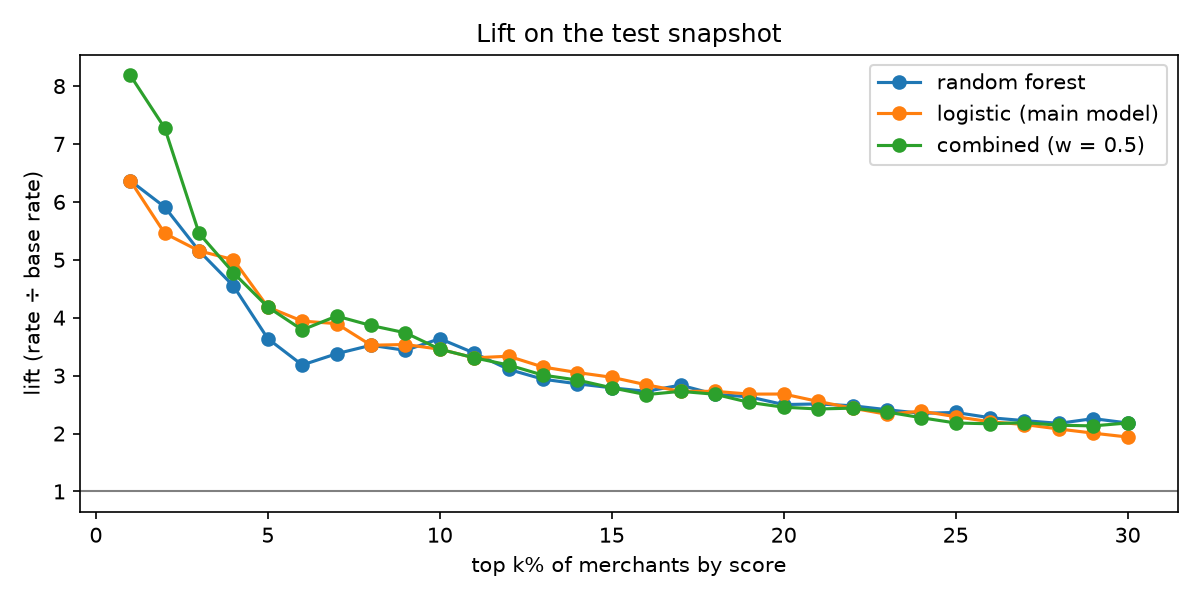
\includegraphics[width=0.8\textwidth]{figures/lift_logistic_rf.png}
\caption{Lift curve of the two models and their combination on the test snapshot.}
\label{fig:lift}
\end{figure}

From the table and the lift curve, both models rank merchants far better than random. The base adoption rate is 1.0\% in 90 days; among the top 1\% of merchants it rises to 6.4\% for both models, and among the top 100 to 7\%. Combining them raises these rates to 8.2\% and 9\%, because the two models make partly different errors; the gain is about two adopters and is limited to the top few percent, beyond which all curves coincide. The moderate AUC of 0.73 reflects that adoption is rare and that the covariates describe only payment volumes and a coarse merchant profile over a short history.

Each model outputs a ranked list of the top 100 merchants at risk on the day after the data ends, with their predicted scores: \code{output/target\_list\_time.csv} (logistic regression) and \code{output/target\_list\_time\_rf.csv} (random forest); the final list from the combined score is described in Section~\ref{sec:lists}.

\subsection{Who adopts}

Table~\ref{tab:odds} shows the main odds ratios of the logistic regression.

\begin{table}[H]
\centering
\caption{Main odds ratios of the logistic regression, with 95\% confidence intervals and p-values from standard errors clustered by merchant.}
\label{tab:odds}
\begin{tabular}{lrrr}
\toprule
Covariate & Odds ratio & 95\% CI & p-value \\
\midrule
Industry: Business services (vs Others) & 3.08 & (2.16, 4.40) & $<0.001$ \\
Industry: Personal services & 2.74 & (1.79, 4.21) & $<0.001$ \\
Industry: Education & 2.26 & (1.35, 3.78) & 0.002 \\
Industry: Software & 2.08 & (1.26, 3.46) & 0.004 \\
Payment Links volume (per unit of log volume) & 1.11 & (1.05, 1.17) & $<0.001$ \\
Active rate (0 to 1) & 0.35 & (0.19, 0.65) & 0.001 \\
Business size: medium/large (vs small) & 0.35 & (0.15, 0.85) & 0.020 \\
Tenure (per unit of log days) & 0.79 & (0.70, 0.88) & $<0.001$ \\
\bottomrule
\end{tabular}
\end{table}

Both models describe the same profile:
\begin{itemize}
  \item \textbf{Service businesses.} Business services, Personal services, Education and Software merchants adopt about two to three times as often as others; their revenue is naturally recurring.
  \item \textbf{Payment Links users.} They already send payment links by hand, which is exactly what Subscriptions automates.
  \item \textbf{Active but not every day.} A periodic billing pattern, unlike retail merchants who sell every day.
  \item \textbf{Small merchants} adopt more often than medium and large ones.
  \item \textbf{Newer merchants} adopt more often: each unit increase in log tenure lowers the odds of adoption by about 21\%.
\end{itemize}

\subsection{Target lists}\label{sec:lists}

Figure~\ref{fig:overlap} shows how much the two models' lists overlap. For any list size from 100 to 1,000 merchants, only about 60\% to 67\% of the two models' top merchants are the same, so the models pick partly different merchants and the combined score draws on both.

\begin{figure}[H]
\centering
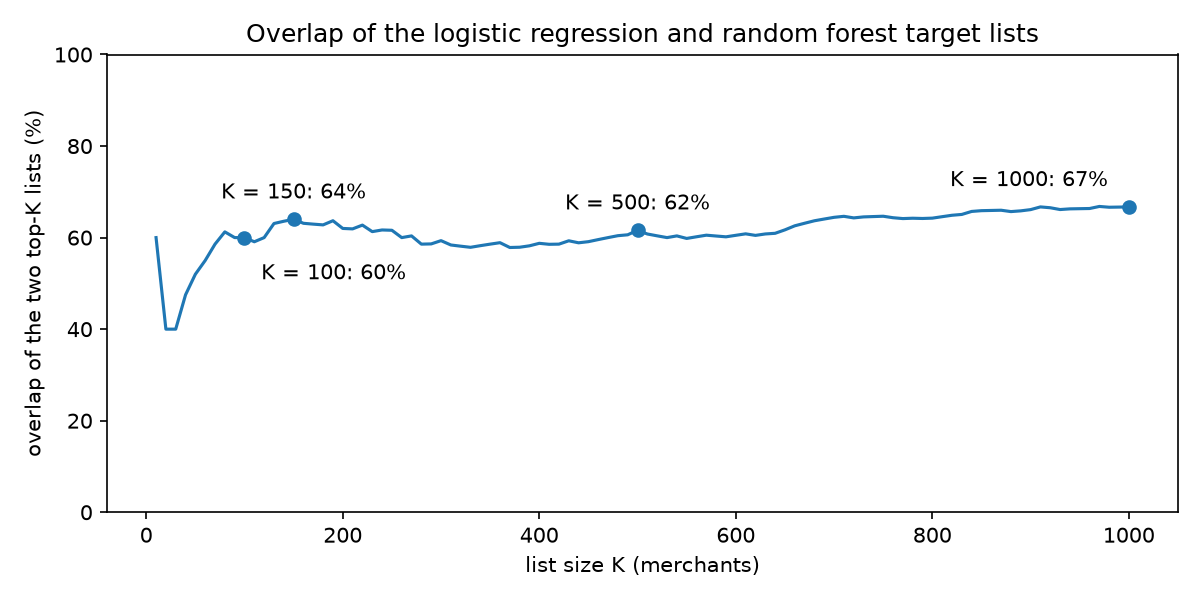
\includegraphics[width=0.8\textwidth]{figures/overlap_logistic_rf.png}
\caption{Overlap of the logistic regression and random forest target lists, by list size.}
\label{fig:overlap}
\end{figure}

The final target list is the top 100 merchants by the combined score (Section~\ref{sec:combine}), saved in \code{output/target\_list\_combined.csv}; it also keeps each model's own score. The two single-model lists overlap on 60 of their 100 merchants, and the combined list shares 77 merchants with the logistic list and 78 with the forest list. \textbf{All 100 are small merchants that use Payment Links, mostly in Business or Personal services.} We would contact them in the order of the combined score. Table~\ref{tab:targets} shows the first 10.

\begin{table}[H]
\centering
\caption{First 10 merchants of the combined target list, with their ranks under each model.}
\label{tab:targets}
\begin{tabular}{lrrr}
\toprule
Merchant & Combined rank & Logistic rank & Random forest rank \\
\midrule
\code{740224c1} & 1 & 2 & 2 \\
\code{67cdfdbd} & 2 & 5 & 3 \\
\code{84627c91} & 3 & 1 & 7 \\
\code{2bd7dae3} & 4 & 3 & 6 \\
\code{a11c5d49} & 5 & 7 & 5 \\
\code{92e17b8d} & 6 & 8 & 10 \\
\code{a0dd9f26} & 7 & 13 & 11 \\
\code{fa0c65ad} & 8 & 9 & 21 \\
\code{b84d83d2} & 9 & 17 & 18 \\
\code{1ec4f633} & 10 & 22 & 13 \\
\bottomrule
\end{tabular}
\end{table}

%--------------------------------------------------------------------
\section{Why not hazard models}\label{sec:hazard}

We did not use hazard models, which model the time until a merchant adopts, because they ranked merchants about as well as the logistic regression while adding assumptions and complexity.
\begin{itemize}
  \item \textbf{Discrete-time hazard model.} A logistic regression on merchant-period data, very close to our rolling-snapshot model.
  \item \textbf{Cox proportional hazards model.} Covariates are fixed at entry, so it ignores changes in behavior, and it relies on proportional hazards.
  \item \textbf{Time-varying Cox model.} It lets covariates change over time, but links the hazard at each moment to the covariates at that moment, whereas we predict future adoption from what we know today; this needs assumptions about future covariates.
\end{itemize}

Our choice of models is based on our understanding of the data and of the campaign; it does not mean that these models are the best possible, or that their assumptions hold exactly.

%--------------------------------------------------------------------
\section{How the company should use it}\label{sec:use}

We recommend using the combined ranking to prioritize merchants for the sales or marketing campaign.
\begin{itemize}
    \item \textbf{Target selection.}
    Rank merchants by their combined score, expanding the list as campaign capacity allows.

    \item \textbf{Channel.}
    Since most selected merchants are small businesses, scalable marketing may be more suitable than individual sales outreach.
    Larger merchants could receive personalized outreach based on their expected value.

    \item \textbf{Campaign execution.}
    Tailor outreach by country or region, industry, and product usage.
    For example, adapt messaging to local markets, highlight industry-specific use cases, and promote recurring billing to Payment Links users.
    Rescore merchants monthly using updated activity.

    \item \textbf{Business value.}
    With calibrated adoption probabilities and merchant value estimates, the company could prioritize merchants by expected adoption-related value.

    \item \textbf{Evaluation.}
    Randomly hold out some target merchants and compare their adoption rates with those contacted to estimate the campaign's incremental effect, using an evaluation period appropriate for the campaign.
\end{itemize}

%--------------------------------------------------------------------
\section{Next steps}\label{sec:next}

\begin{itemize}
  \item \textbf{Randomized experiment and uplift modeling.}
  Estimate the campaign's causal effect over an appropriate evaluation period, then identify merchants most responsive to outreach.

  \item \textbf{Monitoring and retraining.}
  Track calibration, AUC, lift, and covariate drift, and retrain as new outcomes become available.

  \item \textbf{Additional data.}
  Incorporate product usage, recurring-payment patterns, and past sales interactions.

  \item \textbf{Value-based targeting.}
  Combine estimated campaign uplift, merchant value, and outreach costs to maximize expected return.

  \item \textbf{Further modeling and combinations.}
  Explore additional models, such as gradient boosting and survival models, and compare alternative ensemble methods, including weighted rank averaging and stacking, using temporal cross-validation.

  \item \textbf{Campaign simulation.}
  Compare campaign sizes and targeting strategies under different assumptions about outreach effectiveness and costs.
\end{itemize}

%--------------------------------------------------------------------
\section*{Code}

\begin{table}[H]
\centering
\resizebox{\textwidth}{!}{%
\begin{tabular}{llll}
\toprule
Notebook & Role & Input & Output \\
\midrule
\code{data\_cleaning.ipynb} & Read and clean the raw files & Raw merchants (xlsx, csv) and payments (xlsx) & \code{output/merchant\_day.pkl} \\
\code{covariates.ipynb} & Covariate distributions and class decisions & \code{output/merchant\_day.pkl} & \code{output/merchant\_covariates.pkl} \\
\code{logistic.ipynb} & Logistic regression and target list & \code{merchant\_day.pkl}, \code{merchant\_covariates.pkl} & \code{output/target\_list\_time.csv} \\
\code{rf.ipynb} & Random forest, combined model and target lists & \code{merchant\_day.pkl}, \code{merchant\_covariates.pkl} & \code{output/target\_list\_time\_rf.csv}, \code{output/target\_list\_combined.csv} \\
\bottomrule
\end{tabular}%
}
\end{table}

\end{document}
